\chapter{Implementácia}
\label{kap:implementacia}

V kapitole opisujeme priebeh vzniku aplikácie, implementačné detaily, postupy a rozhodnutia. Základné členenie obsahu je podľa modulov, za ktoré považujeme celky aplikácie ako editor kódu v grafickom jazyku, modul pre sériovú komunikáciu či modul pre simuláciu. V rámci jednotlivých častí je opísaný ich vývoj pokiaľ možno chronologicky. Súčasťou sú tiež implementačne zmeny v riadiacich programoch robotov.

\section{Desktopová aplikácia}
Vývoj sme začali návrhom kostry a vizuálnej podoby aplikácie, v ktorej neskôr vznikli jednotlivé moduly. V prvej fáze sme implementovali časti podporujúce komunikáciu s aktuálnou verziou riadiaceho programu robota Otto a jeho programovanie. Nasledovala etapa rozširovania funkcionalít (hlavne grafického jazyka) tak, aby sme sa čo v najväčšej miere vyrovnali existujúcim programom. Súčasne sa zameriavame na modul simulácie.

% GUI
\subsection{Grafické rozhranie}
GUI aplikácie tvoríme pomocou JavaFX. Cieľom je vytvoriť prehľadné prostredie, v ktorom sa ľahko zorientuje i požívateľ nižšieho veku. Pri rozmiestňovaní jednotlivých prvkov sú nám nápomocné existujúce aplikácie, no zohľadňujeme i rady autorov knižnice Blockly \cite{blocklyBestPractices}, keďže komponent umožňujúci prostredníctvom nej programovať robota je v našej aplikácii dominantným. Z odporúčaní je zrejmé, že plochu pre manipuláciu s prvkami grafického jazyka je žiaduce maximalizovať a neoddeľovať ju od komponentu umožňujúceho tvorbu blokov (prvkov jazyka).

Ďalšie prvky vyžadujúce v aplikácii väčšiu plochu sú najmä výstupné, predovšetkým ide o výstup pre modul simulácie a výstup \uv{prekladača} grafického jazyka na kód následne kompilovaný a odosielaný do riadiacej jednotky robota. Taktiež je nutné zakomponovať do GUI modul pre komunikáciu s robotom, konzolu sériovej komunikácie.

Výsledné rozloženie môžete vidieť na obrázku \ref{obr:gui-layout}. Tvoriť kód v grafickom jazyku možno v časti \textit{A}, umožňujúcej výber blokov, a ich následným umiestňovaním v priestore \textit{B}. Sektor \textit{C} je vyhradený pre výstup modulu simulácie. Časť \textit{D} je zdieľaná modulom sériovej komunikácie a modulom umožňujúcim náhľad do kódu generovaného prekladom grafického jazyka, medzi ktorými možno prepínať. Nad spomínanými oblasťami sa nachádza lišta nástrojov, sprístupňujúcich funkcie ako pripojenie a vyhľadanie sériového portu, spustenie simulácie, či voľbu verzie programovaného riadiaceho programu robota.

Prípadná zmena usporiadania komponentov nie je v JavaXF zdĺhavou záležitosťou a na základe spätnej väzby od budúcich používateľov možno v rozložení dodatočne vykonať úpravy.

\begin{figure}
\centerline{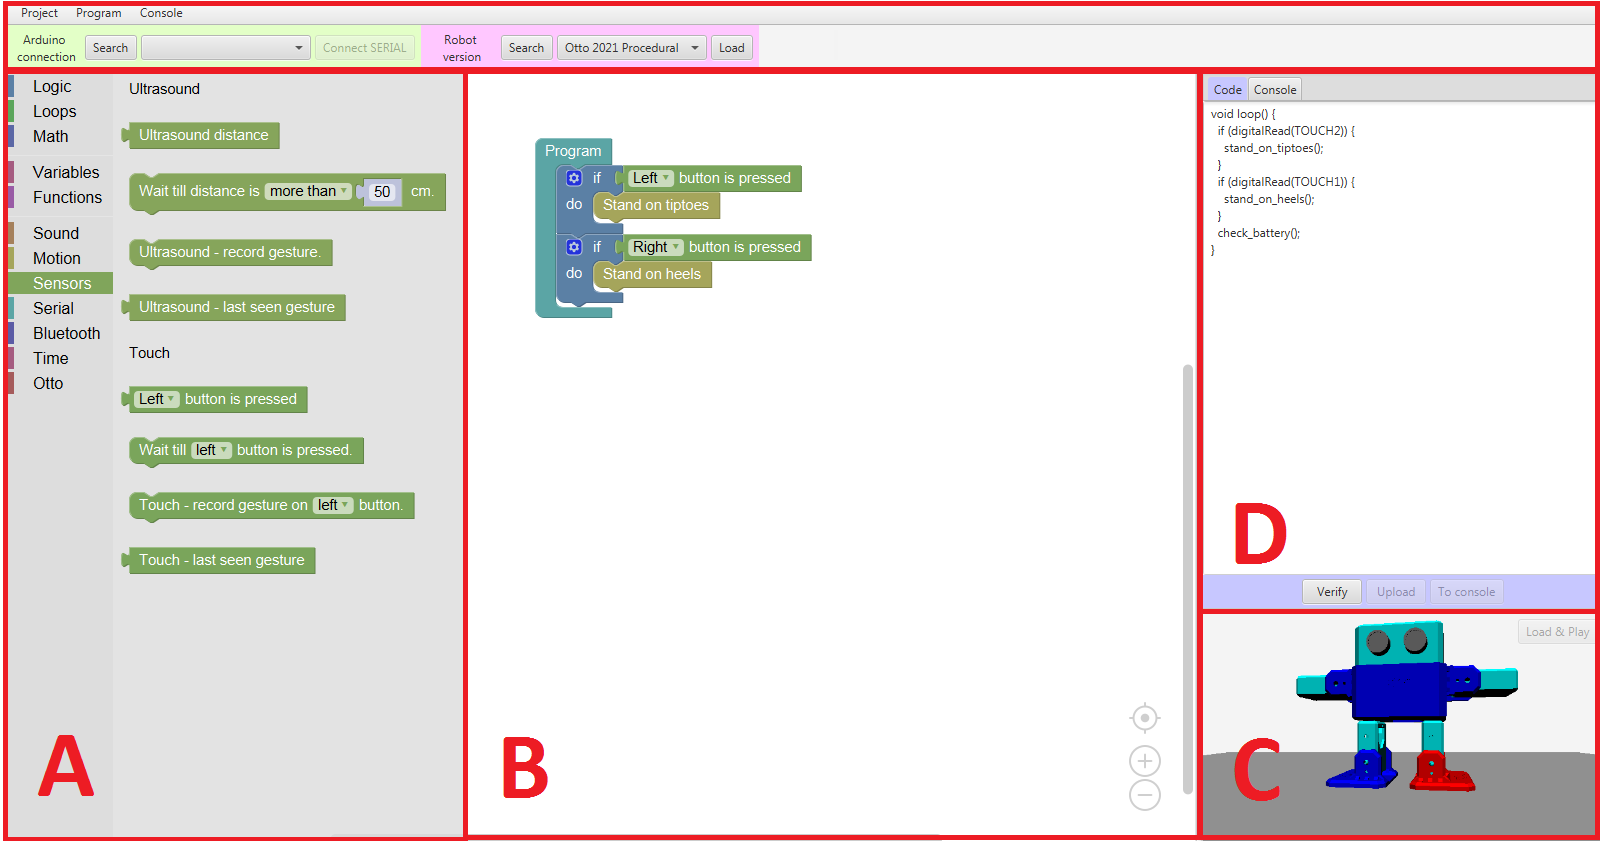
\includegraphics[width=0.4\textwidth]{images/rozlozenie-gui}}
\caption[Rozloženie používateľského rozhrania]{Rozloženie používateľského rozhrania}
\label{obr:gui-layout}
\end{figure}


% Editor kódu
\subsection{Editor kódu}
aka blokové paradigmy, odporúčania tvorcov, uvedomiŤ si kto je publikum, šetriť s počtom blokov, zobraziť len tie čo sa aktuálne dajú použiť

\subsubsection{Obrazový programovací jazyk}
- granularita puzzle
- pre rozne vekove kategorie (na zaklade poziadaviek)
- premenne - problem s typmi

\subsection{Komunikácia s robotom}
todo

\subsubsection{Upload programu}
todo

\subsubsection{Komunikácia cez konzolu}
todo, to co poskytuje putty alebo Arduino IDE, alebo OttoBlockly

\subsection{Kompilácia}
todo

\subsection{Vizualizácia}
todo, tinkerpad, 3d tlac - existujuce modely
- 1.pokus: zobrazenie fixne, rotacia jednotlivych casti
- problemy s fyzikou, komplexita mesh collision shape -> riesenie je boxCollisionShape
- jonts = servo?
- obrazky - motor 130 deg.

\begin{figure}
\centerline{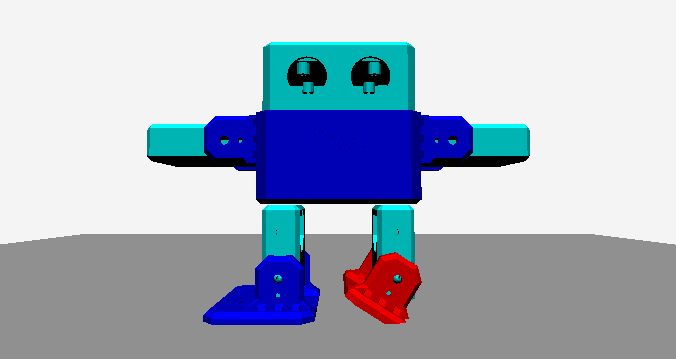
\includegraphics[width=0.4\textwidth]{images/otto-without-collision}}
\caption[Robot Otto - simulácia bez detekcie kolízií]{Robot Otto - simulácia bez detekcie kolízií}
\label{obr:otto-without-collision}
\end{figure}

\begin{figure}
\centerline{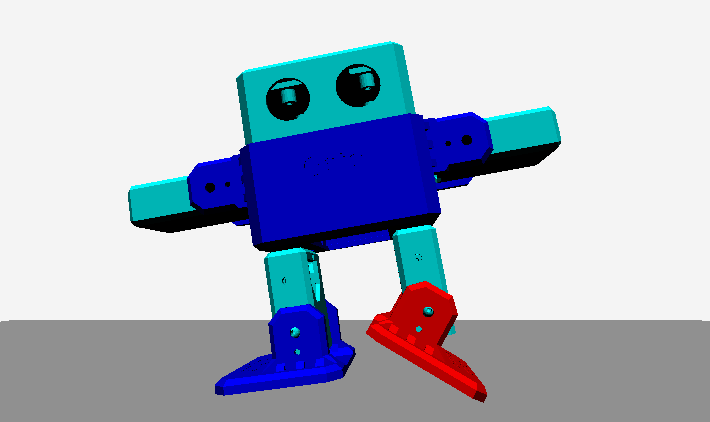
\includegraphics[width=0.4\textwidth]{images/otto-with-collision}}
\caption[Robot Otto - simulácia s detekciou kolízií]{Robot Otto - simulácia s detekciou kolízií}
\label{obr:otto-with-collision}
\end{figure}

\section{Riadiaci program robota}
todo

\subsection{Robot Otto}
todo

\subsection{Robot Mokrarosa}
todo
